
\documentclass{article}

\usepackage{amssymb}
\usepackage{amsmath}

\usepackage[dvips]{graphicx}

\begin{document}

\noindent 

\noindent 

\noindent 

\noindent 



 

\noindent 

\noindent  Software Requirements Specification

\noindent   Squirrel Marking System

\noindent   Version: 1.0

\noindent 

\noindent Organization:

\noindent University of Pretoria: Group 3

\noindent  GitHub:

\noindent  

 https://github.com/Roach-301/CS301\_Group3 

\noindent 

\noindent Authors:

\noindent Johan Esterhuyse (10043283)

\noindent Tokologo Machaba (12078027)

\noindent Heelin Mistry (10299344)

\noindent Pieter le Roux (1045486)

\noindent Rudiger Roach (11004322)

\noindent Thulasizwe Mavuso (29236259)

\noindent 

\noindent March 13, 2014 

  

\textbf{Contents}





\textbf{1  Software architecture design }??

    1.1  Choices of technologies ??

    1.2  Chosen frameworks ??

    1.3  Chosen protocols ??

    1.4  Chosen libraries ??



\textbf{2  Application design }??

    2.1  Back-end ??

    2.2  Web Application ??

    2.3  Android Application ??



 


\subsection{1  Software architecture design}

 


\paragraph{1.1  Choices of technologies}



The existing web server runs on Apache, therefore our system will continue the use thereof.



Django web server, running on Apache, will be our interface to run on.



Djangos Object Relational Mapper Will be used to persist information to the database.



Django unittest module will be used to perform unit tests with. MySQL server allready runs on the CS server and this existing database will be used to pull information from and store information to.



The android application will be built using JAVA.




\paragraph{1.2  Chosen frameworks}

 Django application server will eventually be the framework onto which the system will be deployed and Djangos bundled Object-Relational mapper will be used to access the database. 


\paragraph{1.3  Chosen protocols}

To send data between objects, it will first be encoded into JSON strings. JSON is an easy to use standard that can be parsed by most programming languages. This will enhance our ability to keep layers seperate from each other and just pass JSON strings between layers. 


\paragraph{1.4  Chosen libraries}

 PDF creation will be done using iTextPDF from itextpdf.com. iTextPDF is open source with implementations on multiple different platforms. It is also licensed to enable re-use by developers.



PDF rendering will be done by using the PDFrenderer library from 

https://github.com/katjas/PDFrenderer. This library is LGPL-2.1 licensed and therefore fine for use by us. The library is written in JAVA and uses JAVA2D to render PDF documents.



To marshall and de-marshall JSON, Apache camel will be used from 

http://camel.apache.org/. This library is fully compatible with java and independent from the transport used.




\subsection{2  Application design}

 


\paragraph{2.1  Back-end}

  

     

     

     

     

     

     

 


\paragraph{2.2  Web Application}

\noindent 

\begin{enumerate}
\item  

\item  

\item  

\item  

\item  \textbf{User Interface Design:}
\end{enumerate}

\noindent Login screen:                        Students Menu:

\noindent \includegraphics*[width=2.70in, height=3.34in, keepaspectratio=false]{image1}   \includegraphics*[width=3.44in, height=3.10in, keepaspectratio=false]{image2}

\noindent 

\noindent 

\noindent 

\noindent 

\noindent 

\noindent 

\noindent 

\noindent 

\noindent 

\noindent 

\noindent 

\noindent 

\noindent 

\noindent 

\noindent 

\noindent 

  Students Marks:     Markers Menu:

\noindent \includegraphics*[width=3.21in, height=3.07in, keepaspectratio=false]{image3}  \includegraphics*[width=3.06in, height=3.06in, keepaspectratio=false]{image4}

\noindent 

\noindent 

\noindent 

\noindent 

  Markers Select:     Markers Update:

\noindent \textbf{\includegraphics*[width=3.26in, height=3.25in, keepaspectratio=false]{image5}  \includegraphics*[width=3.08in, height=3.22in, keepaspectratio=false]{image6}}

\noindent \textbf{}

\noindent 

\noindent 

\noindent 

\noindent 

\noindent 

\noindent 

\noindent 

  Lecturer Menu:     Lecturer Session:

\noindent \textbf{\includegraphics*[width=3.12in, height=2.90in, keepaspectratio=false]{image7}  \includegraphics*[width=3.15in, height=2.92in, keepaspectratio=false]{image8}  }

\noindent \textbf{}

\noindent \textbf{}

\noindent \textbf{}

\noindent \textbf{}

\noindent \textbf{}

  Lecturer Create Session:    Lecturer Assign Marker:

\noindent \textbf{\includegraphics*[width=3.10in, height=3.19in, keepaspectratio=false]{image9}   \includegraphics*[width=3.10in, height=3.22in, keepaspectratio=false]{image10}}

\noindent \textbf{}

\noindent \textbf{}

\noindent \textbf{}

\noindent \textbf{}

\noindent \textbf{}

\noindent \textbf{}

\noindent \textbf{}

\textbf{ }  Lecturer Assign Student:     Lecturer Graph:

\noindent \textbf{\includegraphics*[width=3.05in, height=3.41in, keepaspectratio=false]{image11}    \includegraphics*[width=3.05in, height=3.41in, keepaspectratio=false]{image12}}

\noindent \textbf{}

\noindent \textbf{}

\noindent \textbf{Database Design}
The Database will be centralised to one simple design which will be used by all aspects of the system wherever Database access is required.

\noindent \textbf{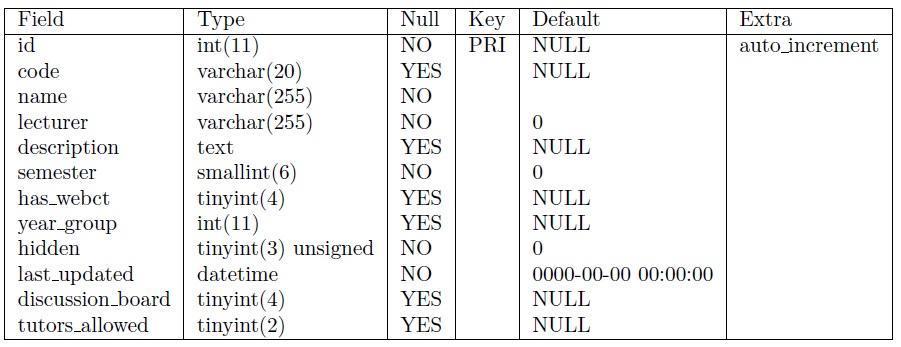
\includegraphics[scale=0.4]{DatabaseDesign.jpg}}

\begin{enumerate}
\item \textbf{ }
\end{enumerate}

\noindent  

\noindent 

\noindent 

\noindent 

\noindent 


\paragraph{2.3  Android Application}

\noindent 

\begin{enumerate}
\item  \textbf{The specifications of lower levels of granularity}
\end{enumerate}

 

\noindent The android application

\begin{enumerate}
\item  Users will also have to be able to login to the application using their CS details. Users that should be able to use the application are markers, lecturers and students (who have android smart phones) 
\end{enumerate}

\noindent 

\noindent Students: 

\begin{enumerate}
\item  Students should be able to check their marks with the android application. 
\end{enumerate}

\noindent 

\noindent Markers: 

\begin{enumerate}
\item  After logging in markers will be able to insert the marks of students that have been assigned to them, for the subject they are marking. They should only be able to insert marks during the practical session (unless otherwise stated). 

\item  Markers can edit student marks but only for a reasonable circumstance. 

\item  Markers can search for students by student number, name and surname.

\item  Marks will be saved locally between updates to the server, so if anything happens to the application or the phone information will be saved, therefore no need to reinsert data already done
\end{enumerate}

\noindent 

\noindent Lecturers: 

\begin{enumerate}
\item  Lecturers should be able to login and choose between a menu of creating a session or viewing marks.

\item  When creating a session, a day, time and duration of the session should be assigned

\item  When assigning students and markers to session, they can be searched for by using student numbers, names and surnames. Multiple students can be assigned to a session by marking the students with a radio button.

\item  After assigning students and markers information should be saved locally between updates to the server.
\end{enumerate}

\noindent 

\noindent 

\begin{enumerate}
\item  The system should log out after no more than 10 minutes of not being used. 

\item  The mobile uses MySQL database which it interacts with via the server. 

\item  Updates between the application and the server should be saved locally on the mobile memory.

\item  When a mark is sent to the system it should be checked to see if it was actually inserted, if not it should try again, if repeated failures are encountered an exception should be thrown telling the user to either retry or try to upload the marks later. 

\item  Mark sheets should lock after the practical session has ended, so that no more marks can be inserted (unless otherwise stated). 
\end{enumerate}

\noindent 

\begin{enumerate}
\item  

\item  

\item  
\end{enumerate}

\noindent \textbf{API Specifications}
In the Android application the markers will be handling the marks as shown below:
\noindent \textbf{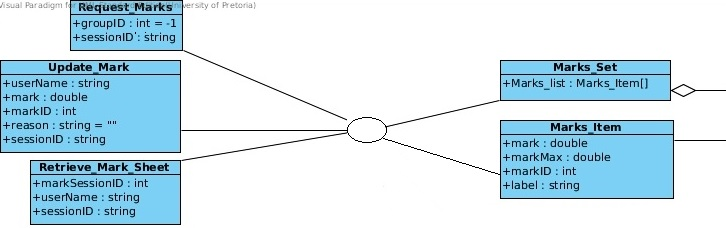
\includegraphics[scale=0.4]{marks.jpg}}

\noindent \textbf{Class Diagrams}
The Android Application will have the following structure: 
\noindent \textbf{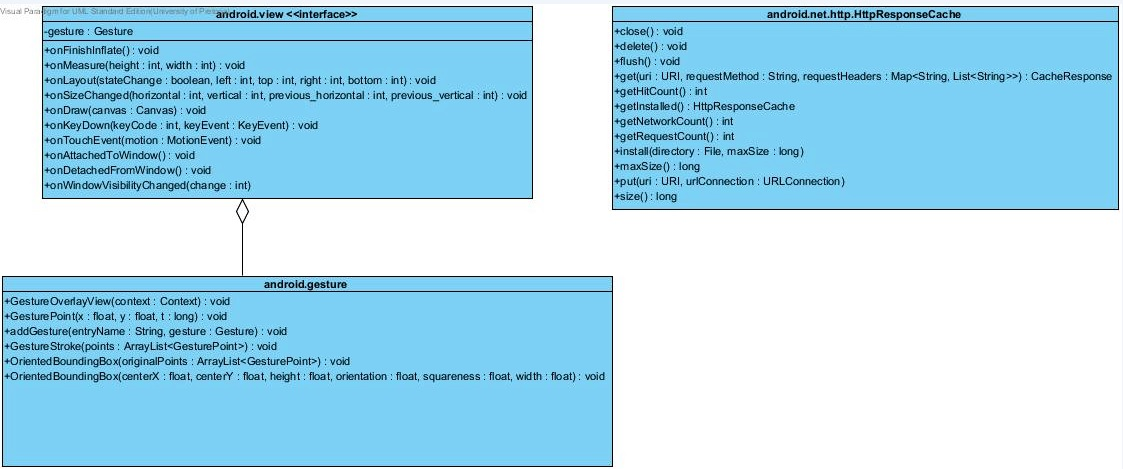
\includegraphics[scale=0.4]{androidClass.jpg}}
Source:
\usepackage{hyperref}
\url{http://developer.android.com/}
\noindent \textbf{System Process Specifications}
Login activity Diagram:
\noindent \textbf{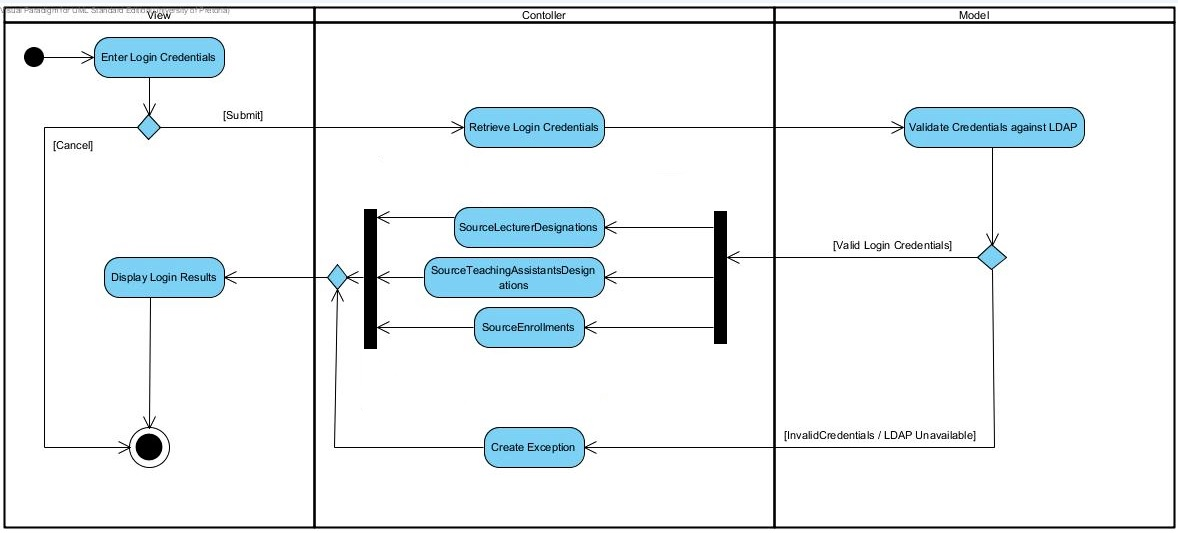
\includegraphics[scale=0.4]{androidLogin.jpg}}
\noindent \textbf{}

\noindent \textbf{}

\noindent \textbf{}

\noindent \textbf{}

\noindent \textbf{}

\noindent \textbf{}

\noindent \textbf{}

\noindent \textbf{}

\noindent \textbf{}

\noindent \textbf{}

\begin{enumerate}
\item \textbf{ User Interface Design:}
\end{enumerate}

\noindent \textbf{}

          Login screen:                        Students Menu:

\includegraphics*[width=2.79in, height=4.01in, keepaspectratio=false]{image13}  \includegraphics*[width=2.82in, height=4.11in, keepaspectratio=false]{image14}  

  Students Marks:              Markers Menu:

\noindent \includegraphics*[width=2.74in, height=4.04in, keepaspectratio=false]{image15}     \includegraphics*[width=2.81in, height=4.07in, keepaspectratio=false]{image16}

  Markers Select:     Markers Update:

\noindent \includegraphics*[width=2.78in, height=4.06in, keepaspectratio=false]{image17}     \includegraphics*[width=2.73in, height=4.04in, keepaspectratio=false]{image18}

\noindent 

\noindent 

\noindent            Lecturer Session:       Lecturer Menu:

\noindent \includegraphics*[width=2.78in, height=4.10in, keepaspectratio=false]{image19}      \includegraphics*[width=2.72in, height=4.06in, keepaspectratio=false]{image20}      

  Lecturer Create:     Lecturer Assign:

\noindent \includegraphics*[width=2.87in, height=4.28in, keepaspectratio=false]{image21}       \includegraphics*[width=2.83in, height=4.19in, keepaspectratio=false]{image22}     

\noindent 

     Lecturer Graphs:

\noindent \includegraphics*[width=2.75in, height=4.09in, keepaspectratio=false]{image23}  

\includegraphics*[width=5.37in, height=9.02in, keepaspectratio=false]{image24}Workflow:











































Workflow:



\noindent 

\noindent 


\end{document}


